\documentclass[../compilation_of_summaries/all_summaries.tex]{subfiles}
\begin{document}
	In \cite{Shou2007} the authors develop a synthetic obligatory cooperating system of two non-mating (naturally non-interactive) yeast cell populations. The authors engineer two straings of Saccharomyces cerevisiae with different metabolic capabilities. The first strain, called R, requires adenine to grow but synthesis lysine at normal levels. The second straing, called Y, requires lysine to grow but produces adenine at normal levels. Thus, without intervention both strains become extinct in isolation. 
	
	The authors found that it is necessary for each strain to overproduce its respective enzyme for cooperation to be successful. This was achieved by removing the natural end-product feedback inhibition system in each culture. The authors noted that the intrinsic asymmetric starvation tolerance between the two strains placed constraints that restrict cooperation. The R strain is able to survive much longer than the Y strain without supplementary enzymes. This mismatch caused an initial loss in culture viability. However, after some dead-time (at very low Y cell density) the cooperation becomes effective, see figure \ref{fig:shou2007_popden}.
		\begin{figure}[h]
			\centering
			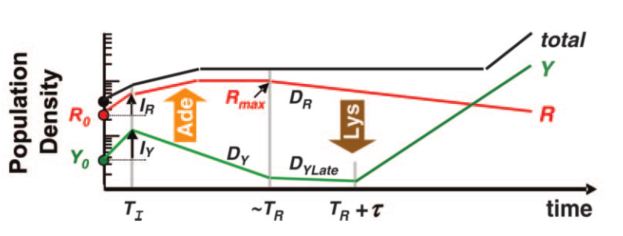
\includegraphics[width=0.8\textwidth]{shou2007_popden.png}
			\caption{Predator Prey gene circuits.}
			\label{fig:shou2007_popden}
		\end{figure}   
	Since the enzymes are only released upon cell death and the R strain can survive for much longer than the Y strain, it was found there existed minimum initial cell density constraints to ensure co-culture viability. Interestingly, the authors found that, irrespective of (viable) initial conditions, the co-cultures converged to a single stable population density ratio. The authors also found, upon long term culturing, the initial cell density required for co-culture viability was reduced. 
\end{document}